\section{Numerical Analysis}
\subsection{Loading/Unloading Criterion}
We present a uniaxial loading--unloading cycle  example to demonstrate the difference between the conventional Kuhn--Tucker condition and the corrected loading/unloading criterion.
The analysis consists of two phases: a loading phase ($0<t<1$) and an unloading phase ($1<t<2$).

\begin{figure}[H]
\centering
\begin{subfigure}{.48\textwidth}
\centering
\includegraphics[page=7]{PICCOLLECTION}
\caption{normal yield ratio}\label{fig:compare_loading_criterion_z}
\end{subfigure}\hfill
\begin{subfigure}{.48\textwidth}
    \centering
    \includegraphics[page=8]{PICCOLLECTION}
    \caption{accumulated plastic strain}\label{fig:compare_loading_criterion_q}
\end{subfigure}
\caption{correct loading criterion accumulates plasticity even when normal yield ratio decreases within the given step}\label{fig:compare_loading_criterion}
\end{figure}
For the amplified step shown in \figref{fig:compare_loading_criterion}, the applied load increment reverses the loading direction, yielding a subloading surface that is smaller than the one at the beginning of the step.
As a result, the normal yield ratio $z$ decreases within the step, as shown in \figref{fig:compare_loading_criterion_z}.
The conventional loading/unloading criterion would simply treat it as a pure elastic unloading step, causing no accumulation of plastic strain as can be seen in \figref{fig:compare_loading_criterion_q}.

On contrary, the loading/unloading criterion discussed in \secref{sec:correct_loading_criterion} accumulates plasticity even when the normal yield ratio decreases within the step, since it corrects the initial value of the normal yield ratio $z$ to the minimum within the step.
\subsection{Error Map}
We follow a standard procedure to compute the error map \citep[see, e.g.,][\S~3.4.4]{Simo1998}.
The loading protocol can be described as follows: for region A (biaxial loading), a strain load ($\varepsilon_x=\varepsilon_y$) is applied until $\varepsilon_x=\varepsilon_y=4\varepsilon^i$, where $\varepsilon^i=\sigma^i/E$; for region B (uniaxial loading), a strain load ($\varepsilon_x$) is applied until $\varepsilon_x=4\varepsilon^i$.
Then different combinations of $\Delta\varepsilon_x,\Delta\varepsilon_y\in[-3\varepsilon^i,3\varepsilon^i]$ are applied in a single step to obtain the numerical stress $\bsigma_\text{num}$.
\figref{fig:error_euler_loading} depicts the region where the error map is computed.
\begin{figure}[htb]
    \centering
    \includegraphics[page=9]{PICCOLLECTION}
    \caption{loading history used in computation of error map}\label{fig:error_euler_loading}
\end{figure}

The errors are computed as
\begin{gather}
    \text{absolute error}=\sqrt{\left(\bsigma_\text{ref}-\bsigma_\text{num}\right):\left(\bsigma_\text{ref}-\bsigma_\text{num}\right)},\\
    \text{relative error}=\dfrac{\text{absolute error}}{\norm{\bsigma_\text{ref}}}\times\SI{100}{\percent},
\end{gather}
where $\bsigma_\text{num}$ is computed using a single load increment (step) and $\bsigma_\text{ref}$ is computed using a very fine time step.
\paragraph{Simple Parameter Set}
We first present a simple example adopting linear isotropic hardening only.
The following parameters are used in the numerical analysis: $E=\SI{2E5}{\mega\pascal}$, $\nu=0.2$, $\sigma^i=\SI{100}{\mega\pascal}$, $k_\text{iso}=\SI{2E3}{\mega\pascal}$, $u=\num{5E2}$.
The rest of the parameters are set to zero.
The corresponding error map is shown in \figref{fig:error_euler_isotropic}.
\begin{figure}[htb]
\centering
\begin{subfigure}{.48\textwidth}\centering
    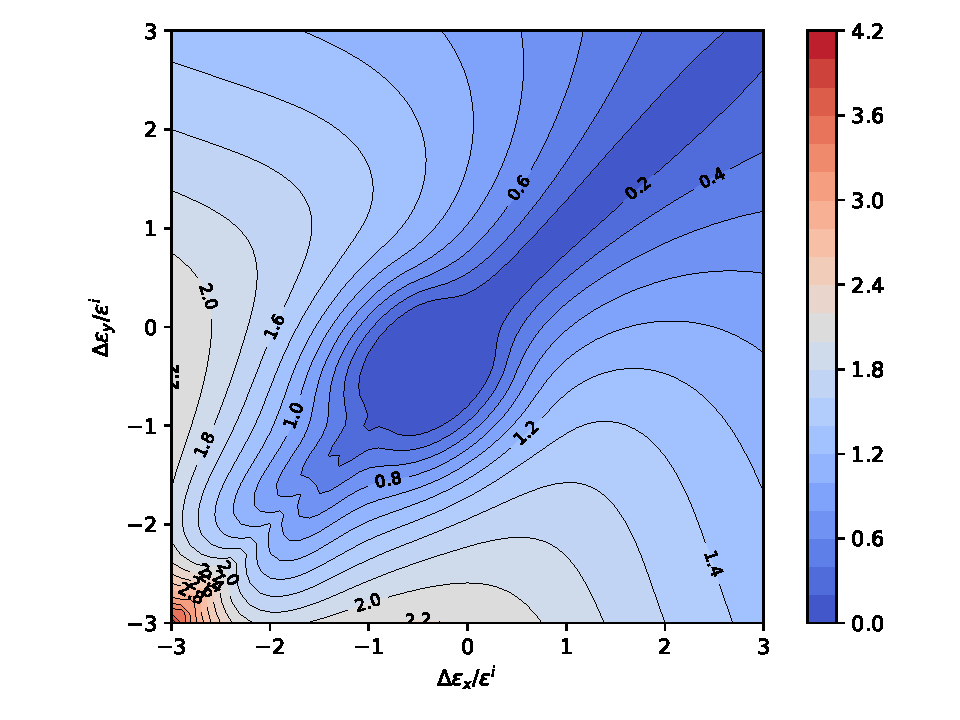
\includegraphics[width=.99\textwidth]{PIC/ISOMAP/error.iso.biaxial.pdf}
    \caption{region A (biaxial)}\label{fig:error_euler_iso_a}
\end{subfigure}\hfill
\begin{subfigure}{.48\textwidth}\centering
    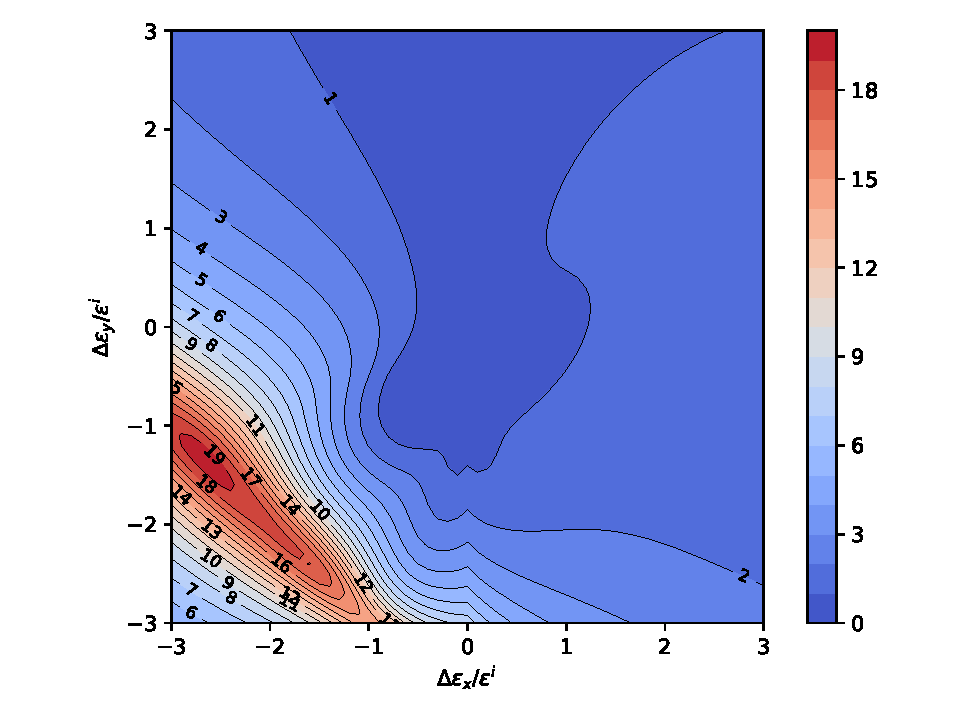
\includegraphics[width=.99\textwidth]{PIC/ISOMAP/error.iso.uniaxial.pdf}
    \caption{region B (uniaxial)}\label{fig:error_euler_iso_b}
\end{subfigure}
\caption{error map (\si{\percent}) using the closest point projection method (isotropic hardening only)}\label{fig:error_euler_isotropic}
\end{figure}
\paragraph{With Elastic Core}
The evolution of elastic core, along with both isotropic and kinematic hardening, is considered in this example.
The following parameters are used in the numerical analysis: $E=\SI{2E5}{\mega\pascal}$, $\nu=0.2$, $\sigma^i=\SI{100}{\mega\pascal}$, $k_\text{iso}=\SI{2E3}{\mega\pascal}$, $u=\num{5E2}$, $a^i=\SI{200}{\mega\pascal}$, $b=\num{5E2}$, $c_e=\num{5E2}$ and $z_e=\num{0.7}$.
The rest of the parameters are set to zero.
The corresponding error map is shown in \figref{fig:error_euler_with_core}.
\begin{figure}[htb]
\centering
\begin{subfigure}{.48\textwidth}\centering
    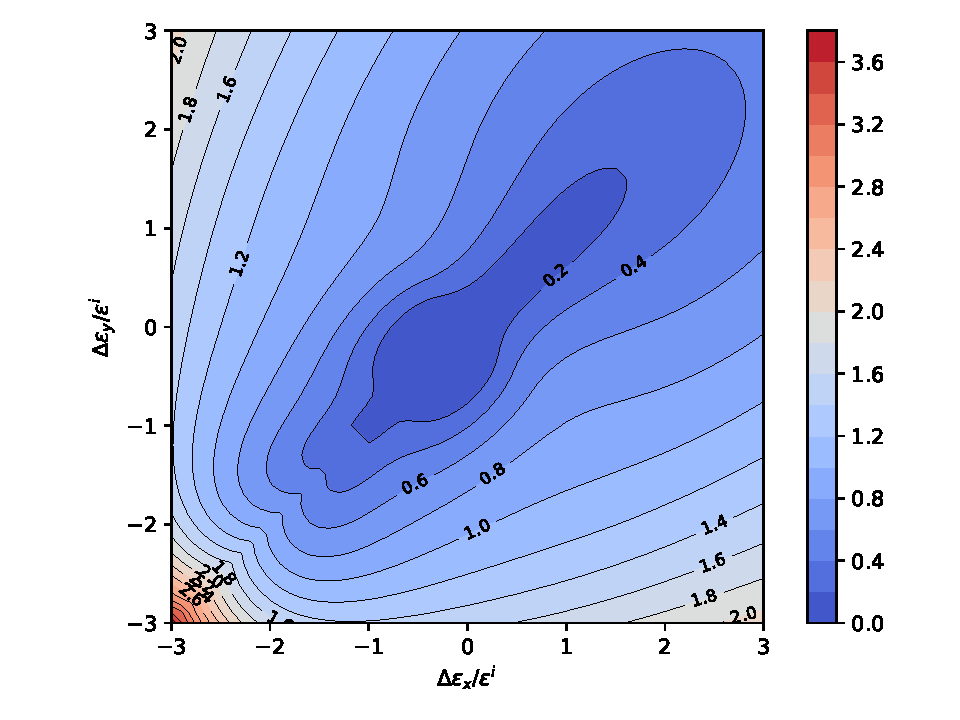
\includegraphics[width=.99\textwidth]{PIC/ISOMAP/error.core.biaxial.pdf}
    \caption{region A (biaxial)}\label{fig:error_euler_with_core_a}
\end{subfigure}\hfill
\begin{subfigure}{.48\textwidth}\centering
    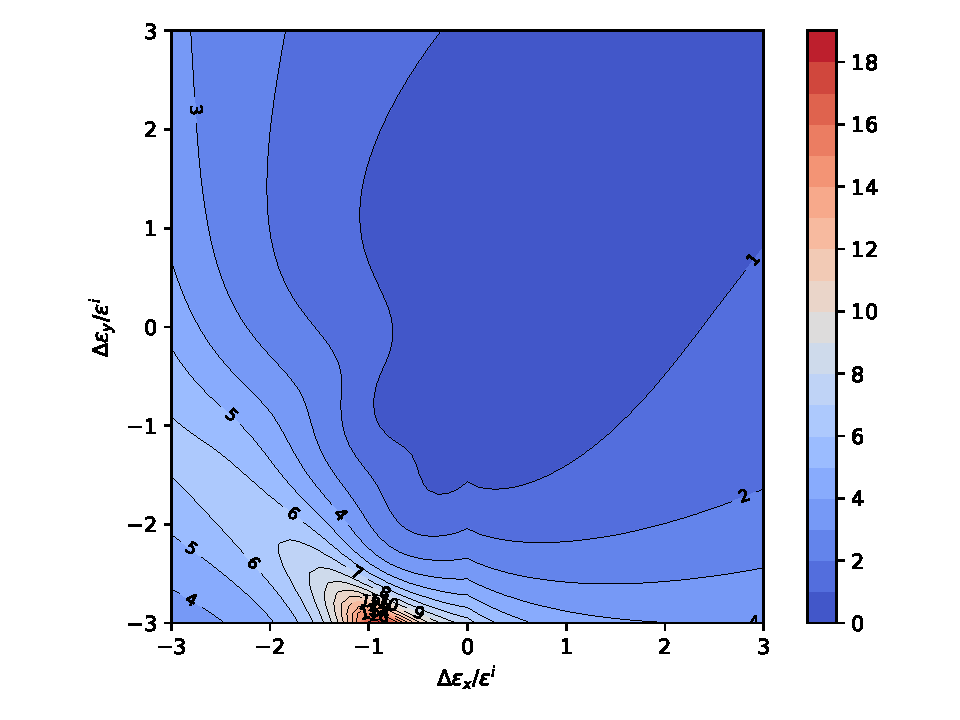
\includegraphics[width=.99\textwidth]{PIC/ISOMAP/error.core.uniaxial.pdf}
    \caption{region B (uniaxial)}\label{fig:error_euler_with_core_b}
\end{subfigure}
\caption{error map (\si{\percent}) using the closest point projection method (with elastic core)}\label{fig:error_euler_with_core}
\end{figure}

For biaxial loading path, it can be observed that the unloading direction (towards the origin) tends to have a higher error than the rest.
For uniaxial loading path, significant errors are observed around the regions where $z$ is close to zero.
The rest of the regions appear to have a relatively good accuracy according to the \SI{5}{\percent} rule \citep[see][pg.~132]{Simo1998}.
% This is mainly caused by the fact that the numerical integration of $z$ is less accurate around $z=0$, especially when the step size is large, as the adopted rate function $U\left(z\right)$ is not bounded and approaches infinity as $z$ approaches zero.
% However, even using a more accurate numerical method, such as the trapezoidal rule, the corresponding numerical performance would not be significantly improved.

In fact, using the indicator adopted by \citet{Anjiki2019}, which is effectively the absolute error, one could see that the large relative error is mainly caused by the small reference stress $\bsigma_\text{ref}$.
\figref{fig:abs_error} further show the absolute error map in region B for the two cases considered.
\begin{figure}[htb]
    \centering
    \begin{subfigure}{.48\textwidth}\centering
        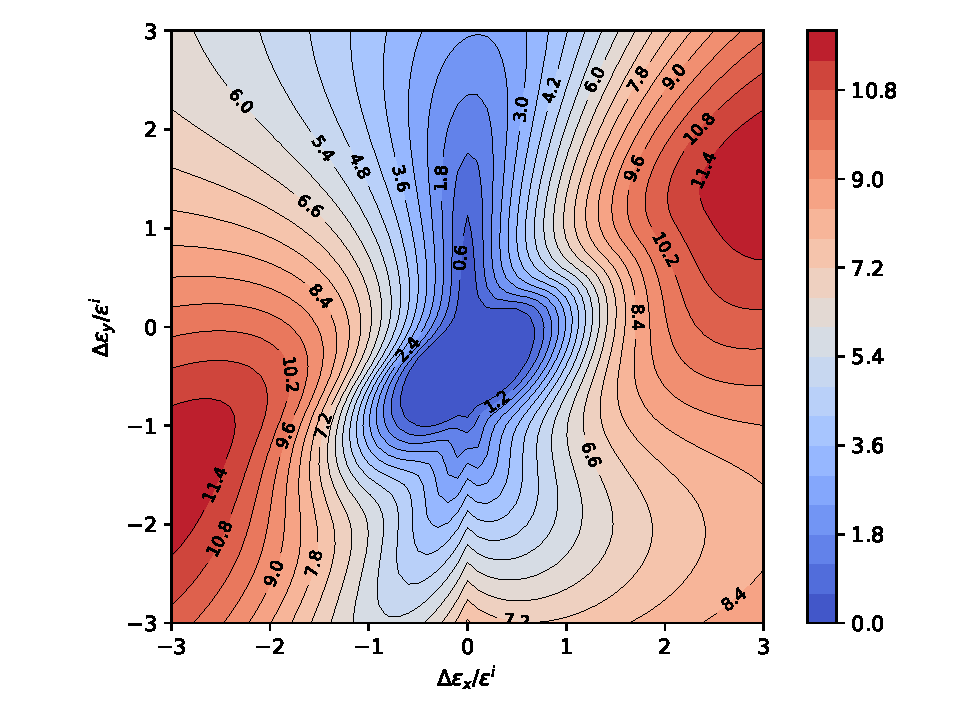
\includegraphics[width=.99\textwidth]{PIC/ISOMAP/abs.error.iso.uniaxial.pdf}
        \caption{with isotropic hardening only}\label{fig:abs_error_euler_with_iso}
    \end{subfigure}\hfill
    \begin{subfigure}{.48\textwidth}\centering
        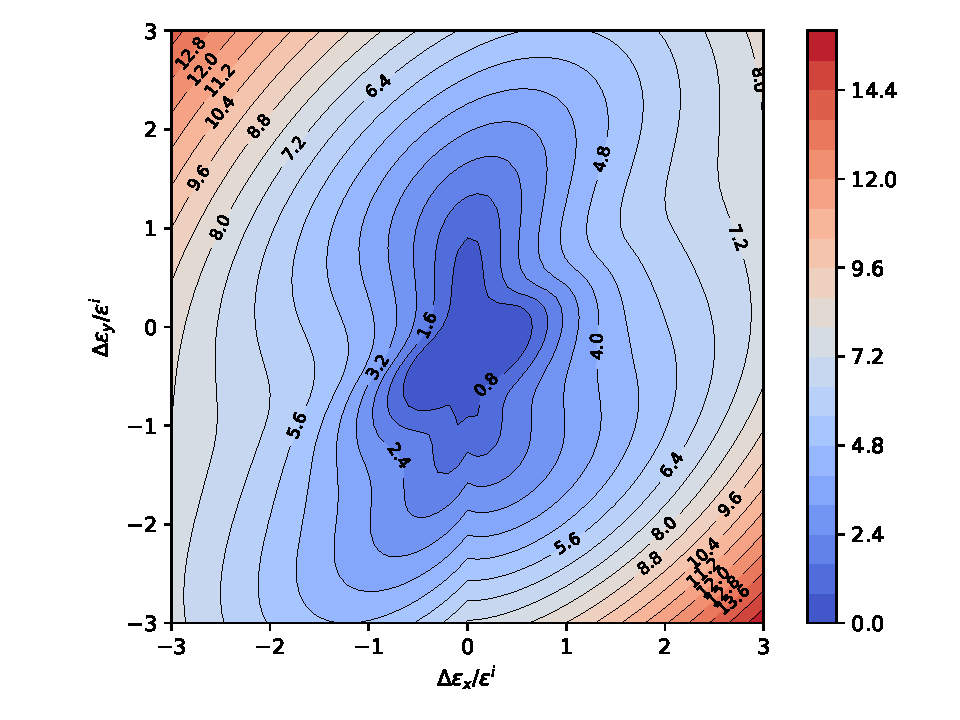
\includegraphics[width=.99\textwidth]{PIC/ISOMAP/abs.error.core.uniaxial.pdf}
        \caption{with elastic core}\label{fig:abs_error_euler_with_core}
    \end{subfigure}
    \caption{absolute error map in region B}\label{fig:abs_error}
\end{figure}
It could be observed that there is no significant difference between outwards and inwards directions.
The overall error is below \SIrange{5}{6}{\percent} of $\sigma^i$ in most regions.
\subsection{Cyclic Response}
The reference comparison can be seen in the work by \citet{Hassan2008,Hashiguchi2017a}.
The following parameters are used:
$E=\SI{2E5}{\mega\pascal}$,
$\sigma^i=\SI{232}{\mega\pascal}$,
$\sigma^s_\text{iso}=\SI{70}{\mega\pascal}$,
$m^s_\text{iso}=\num{30}$,
$a^i=\SI{209}{\mega\pascal}$,
$a^s_\text{kin}=\SI{63}{\mega\pascal}$,
$m^s_\text{kin}=\num{30}$,
$u=\num{2E3}$,
$b=\num{2}$,
$c_e=\num{143}$,
$z_e=\num{0.7}$.
The rest of the parameters are set to zero.

\figref{fig:cyclic_total} depicts the cyclic response.
Due to the presence of the elastic core, the evolution $d$ allows plastic strain to accumulate even when the material undergoes `elastic unloading' (in the conventional sense).
\begin{figure}[htb]
\centering
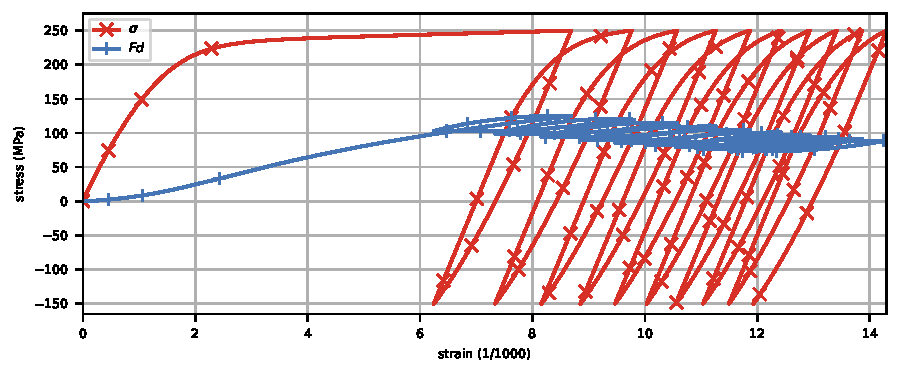
\includegraphics{PIC/CYCLIC/cyclic.total.pdf}
\caption{total stress and evolution of elastic core}\label{fig:cyclic_total}
\end{figure}

\figref{fig:internal_total} and \figref{fig:internal_q} show the evolution of the normal yield ratio $z$ and the similarity vector $d$ against the total strain $\varepsilon$ and the accumulated plastic strain $q$, respectively.
\begin{figure}[htb]
    \centering
    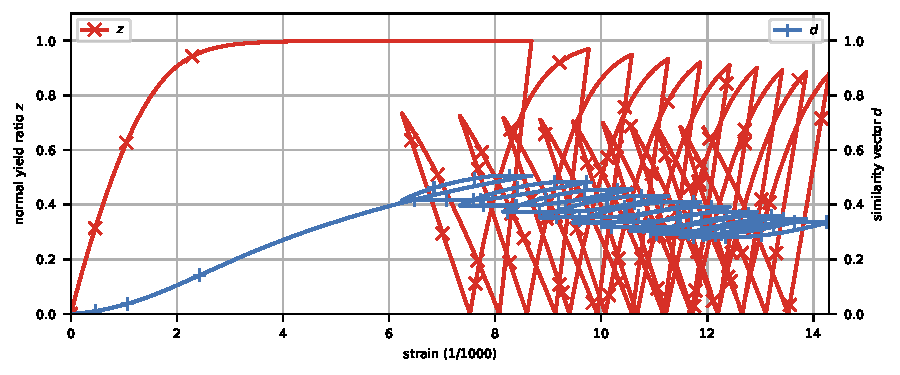
\includegraphics{PIC/CYCLIC/cyclic.ratio.total.pdf}
    \caption{normal yield ratio $z$ and similarity vector $d$ against total strain $\varepsilon$}\label{fig:internal_total}
    \end{figure}
    \begin{figure}[htb]
    \centering
    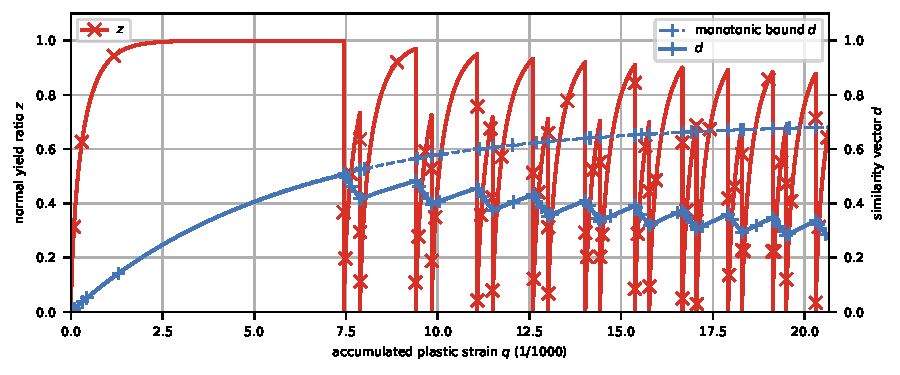
\includegraphics{PIC/CYCLIC/cyclic.ratio.plastic.pdf}
    \caption{normal yield ratio $z$ and similarity vector $d$ against accumulated plastic strain $q$}\label{fig:internal_q}
\end{figure}
Since the model presented in this work is functionally equivalent to the original extended subloading surface model, the overall performance is expected to be similar.
However, as the relevant parameters are defined differently in this work, not all of them are interchangeable with the original model in general.